\documentclass{beamer}
\beamertemplatenavigationsymbolsempty
\usecolortheme{beaver}
\setbeamertemplate{blocks}[rounded=true, shadow=true]
\setbeamertemplate{footline}[page number]
%
\usepackage[utf8]{inputenc}
\usepackage[english,russian]{babel}
\usepackage{amssymb,amsfonts,amsmath,mathtext}
\usepackage{subfig}
\usepackage[all]{xy} % xy package for diagrams
\usepackage{array}
\usepackage{multicol}% many columns in slide
\usepackage{hyperref}% urls
\usepackage{hhline}%tables
\usepackage{subfig}
\usepackage{graphicx}

% Your figures are here:
\graphicspath{ {fig/} {../fig/} }

%----------------------------------------------------------------------------------------------------------
\title[\hbox to 56mm{Состязательные мосты Шрёдингера на задаче трансляции домена}]{Состязательные мосты Шрёдингера на задаче трансляции домена}
\author[Г.\,С.~Ксенофонтов]{Ксенофонтов Григорий Сергеевич\\
\small Научный руководитель: к.ф.-м.н. Р.\,В.~Исаченко}
\institute{Кафедра интеллектуальных систем ФПМИ МФТИ\\
Специализация: Интеллектуальный анализ данных\\
Направление: 03.04.01 Прикладные математика и физика}
\date{2024}

%----------------------------------------------------------------------------------------------------------
\begin{document}
%----------------------------------------------------------------------------------------------------------
\begin{frame}
\thispagestyle{empty}
\maketitle
\end{frame}
%-----------------------------------------------------------------------------------------------------
\begin{frame}{Состязательные мосты Шрёдингера}
    \begin{block}{Задача}
        Найти прямое и обратное отображения между двумя наборами данных с использованием мостов Шрёдингера.
    \end{block}
    \begin{block}{Проблема}
        Современные подходы либо плохо справляются с большой размерностью, либо используют вычислительно трудное моделирование стохастического процесса.
    \end{block}
    \begin{block}{Решение}
        Решить задачу мостов Шрёдингера с помощью состязательного обучения.
    \end{block}
\end{frame}
%-----------------------------------------------------------------------------------------------------
\begin{frame}{Постановка задачи трансляции домена}
Задача трансляции домена заключается в нахождении отображения $G: X \rightarrow Y$
\begin{figure}
    \centering
    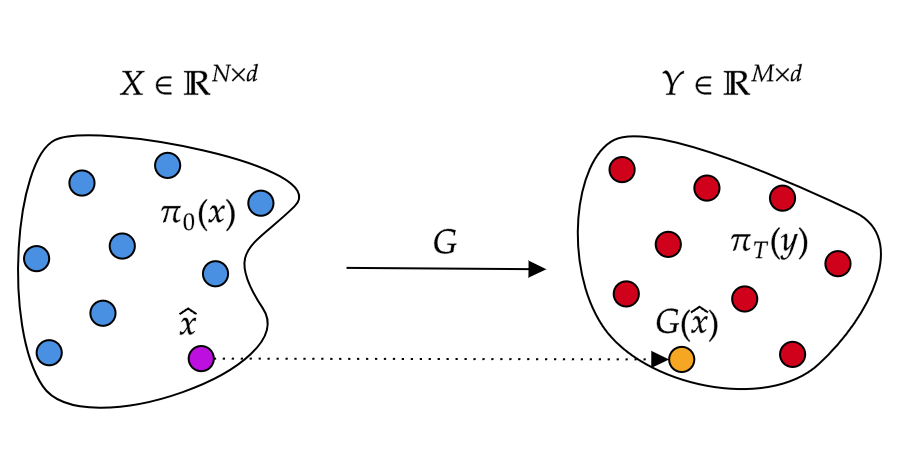
\includegraphics[width=1\linewidth]{slides//4th//figures/translation_task.png}
\end{figure}
\end{frame}


\begin{frame}{Мост Шрёдингера}
Пусть дано:
\begin{enumerate}[1.]
    \item непарные наборы данных $X$ и $Y$;
    \item $p^{\mathbb{W}^{\gamma}}(x_0, \dots, x_T)$ -- совместное распределение Винеровского процесса $\mathbb{W}^{\gamma}$ c коэффицентом волатильности $\sqrt{\gamma}$.
\end{enumerate}
\vfill
Тогда \textbf{мост Шрёдингера}:
\begin{equation*}
    q^*(x_0, \dots, x_T) = \arg\min_{q\in \mathcal{D}(\pi_0, \pi_T)} D_{KL}(q(x_0, \dots, x_T)||p^{\mathbb{W}^{\gamma}}(x_0, \dots, x_T)),
\end{equation*}
где $\mathcal{D}(\pi_0, \pi_T)$ -- множество всех совместных распределений с маргиналами \pi_0(x_0), \pi_T(x_T)

\end{frame}
%----------------------------------------------------------------------------------------------------------
\begin{frame}{Трансляция с помощью моста Шрёдингера}
Для трансляции с помощью мостов Шрёдингера моделируется сопоставленный стохастический процесс заданный следующим СДУ:
\begin{equation*}
    G: dx_t = \underbrace{f(x_t)dt}_{\text{скорость}} + \underbrace{\sqrt{\gamma}d\mathbb{W}_t}_{\text{разнообразие}},
\end{equation*}
где $f: \mathbb{R}^d \rightarrow \mathbb{R}^d$ -- функция смещений, а $\mathbb{W}$ -- винеровский процесс.

\vfill
Эквивалентной задачей мостов Шрёдингера является:
\begin{equation*}
    \min_{q\in \mathcal{D}(\pi_0, \pi_T)}\frac{1}{2\gamma}\mathbb{E}_q\left[\int_0^T||f(x_t)||^2dt\right]
\end{equation*}

Из этого следуют \textbf{преимущества} моста Шрёдингера:
\begin{itemize}
    \item быстрая трансляция, за счет минимизаци $f$;
    \item контроль разнообразие транслированных объектов, за счет выбора $\gamma$.
\end{itemize}
\end{frame}

\begin{frame}{Проблемы и предлагаемое решение}
\begin{alertblock}{Проблемы}
    \begin{enumerate}
        \item Моделирование процесса является вычислительно трудной задачей;
        \item Методы, не моделирующие процесс, страдают от проклятия размерности.
    \end{enumerate}
    
\end{alertblock}

\vfill
\begin{exampleblock}{Решение}
    Перейти к статической постановке задачи мостов Шрёдингера:
    \begin{equation*}
        q^*(x,y) = \arg\min_{q\in \mathcal{D}(\pi_0, \pi_T)} D_{KL}(q(x,y)||p^{\mathbb{W}^\gamma}(x,y)),
    \end{equation*}
    и представить дивергенцию Кульбака-Лейблера в вариационном виде.
\end{exampleblock}

\end{frame}

\begin{frame}{Iterational Proportional Fitting (IPF)}
    Задача мостов Шрёдингера решается с помощью итеративного алгоритма Iterational Proportional Fitting (IPF):
    \begin{align*}
            \underbrace{\min_{p\in \mathcal{D}(\cdot, \pi_T)}D_{KL}(p(x,y)||q^*(x,y))}_\text{\color{red}обратный шаг}; &
            \underbrace{\min_{q\in \mathcal{D}(\pi_0, \cdot)}D_{KL}(q(x,y)||p^*(x,y))}_\text{\color{blue}прямой шаг}
    \end{align*}
    \begin{figure}
        \centering
        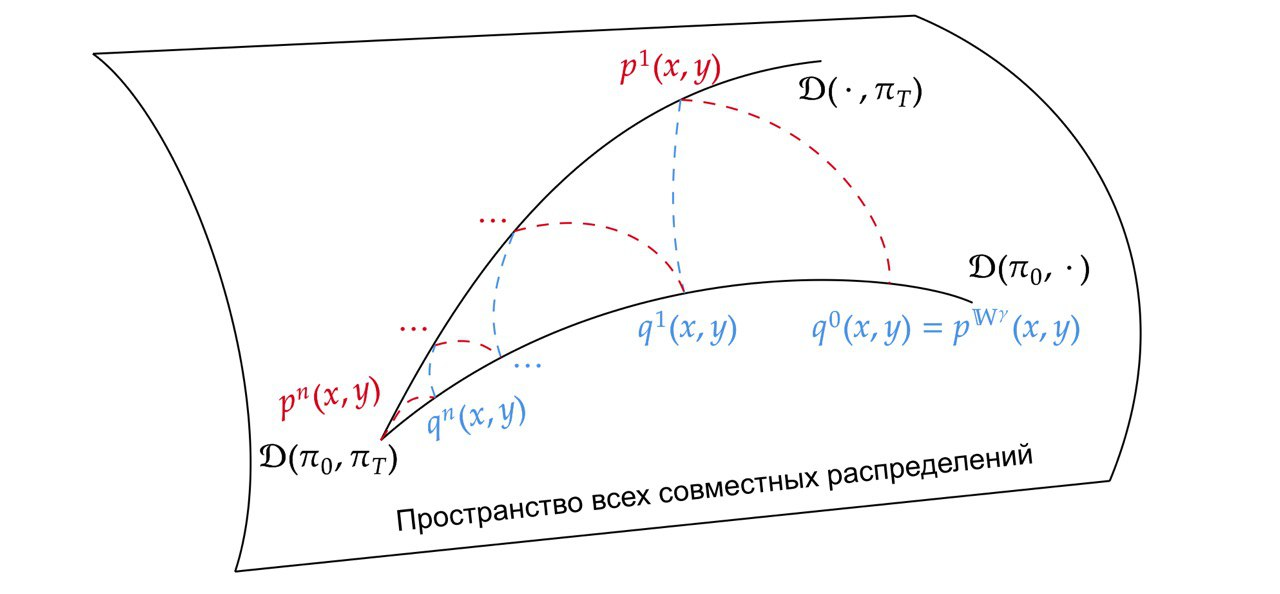
\includegraphics[width=0.9\linewidth]{slides//4th//figures/ipfp.png}
    \end{figure}
\end{frame}

\begin{frame}{Предложенный метод}
    ~\\[-1mm]
    
    \begin{block}{\color{red}Обратный шаг}
        \begin{displaymath}
            \min_{p(x|y)}\max_{D}{\color{violet}\mathbb{E}_{y \sim \pi_T}\mathbb{E}_{x\sim p(x|y)}}\left[D(x,y)\right] - {\color{violet}\mathbb{E}_{x\sim\pi_0}\mathbb{E}_{y\sim q^*(y|x)}}\left[e^{D(x,y) - 1}\right]
        \end{displaymath}
    \end{block}
    \begin{block}{\color{blue}Прямой шаг}
        \begin{displaymath}
            \min_{q(y|x)}\max_{D}{\color{violet}\mathbb{E}_{x \sim \pi_0}\mathbb{E}_{y\sim q(y|x)}}\left[D(x,y)\right] - {\color{violet}\mathbb{E}_{y\sim\pi_T}\mathbb{E}_{x\sim p^*(x|y)}}\left[e^{D(x,y) - 1}\right]
        \end{displaymath}
    \end{block}
    
    \footnotetext[1]{\href{https://arxiv.org/abs/1606.00709}{f-GAN: Training Generative Neural Samplers using Variational Divergence Minimization}}
    \footnotetext[2]{\href{https://arxiv.org/abs/1411.1784}{Conditional Generative Adversarial Nets}}
\end{frame}
%----------------------------------------------------------------------------------------------------------
\begin{frame}{Постановка экспериментов}
    \begin{block}{Эксперимент на 2D данных}
        \begin{itemize}
            \item \textbf{Цель:} санитарное тестирование предложенного метода и сравнение мостов с различной $\gamma$ и с CycleGAN;
            \item \textbf{Данные:} точки из распределений колец, лун, рулета и стандартной гауссианы.
        \end{itemize}
    \end{block}
    \begin{block}{Эксперимент на EMNIST}
        \begin{itemize}
            \item \textbf{Цель:} проверить работоспособность метода на данных большей размерности;
            \item \textbf{Данные:} $X$ --- буквы из EMNIST, $Y$  --- цифры из EMNIST.
        \end{itemize}
    \end{block}
\end{frame}

\begin{frame}{2D данные: санитарное тестирование}
    Данный эксперимент проводился на кольцах, $X$, и лунах, $Y$.
    \begin{figure}
        \centering
        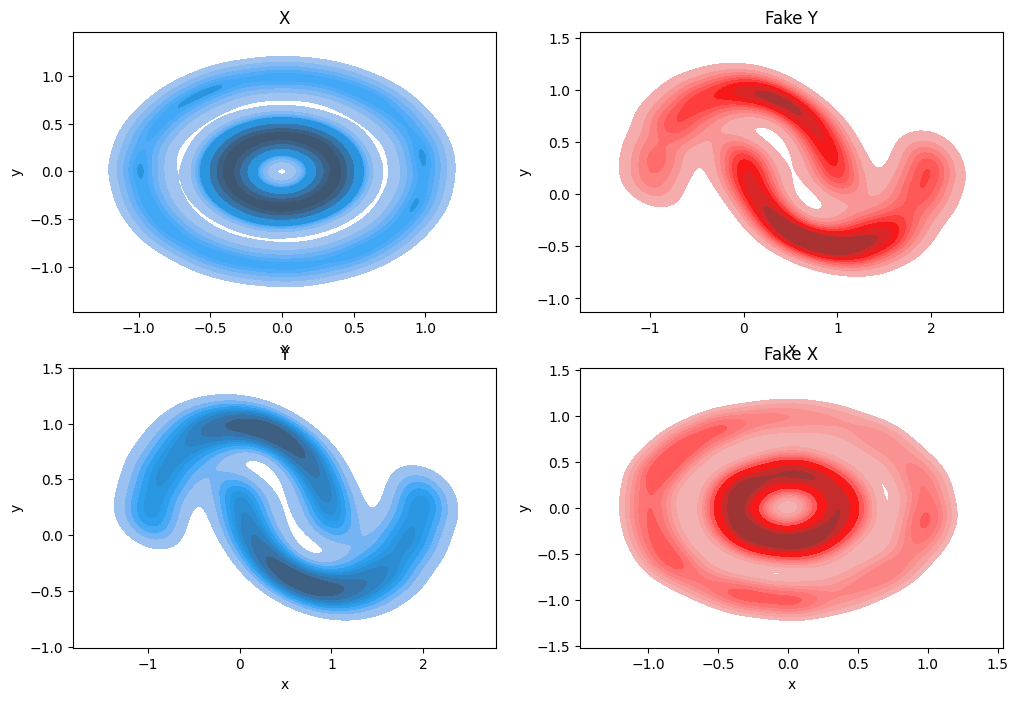
\includegraphics[width=0.9\linewidth]{slides//4th//figures/2d_results.png}
    \end{figure}
\end{frame}


\begin{frame}{2D данные: сравнение мостов с различной $\gamma$}
    Данный эксперимент проводился на стандартной гауссиане, $X$, и рулете, $Y$. Результаты показывают, что предложенный метод справляется с малыми $\gamma$.
    \begin{figure}
        \centering
        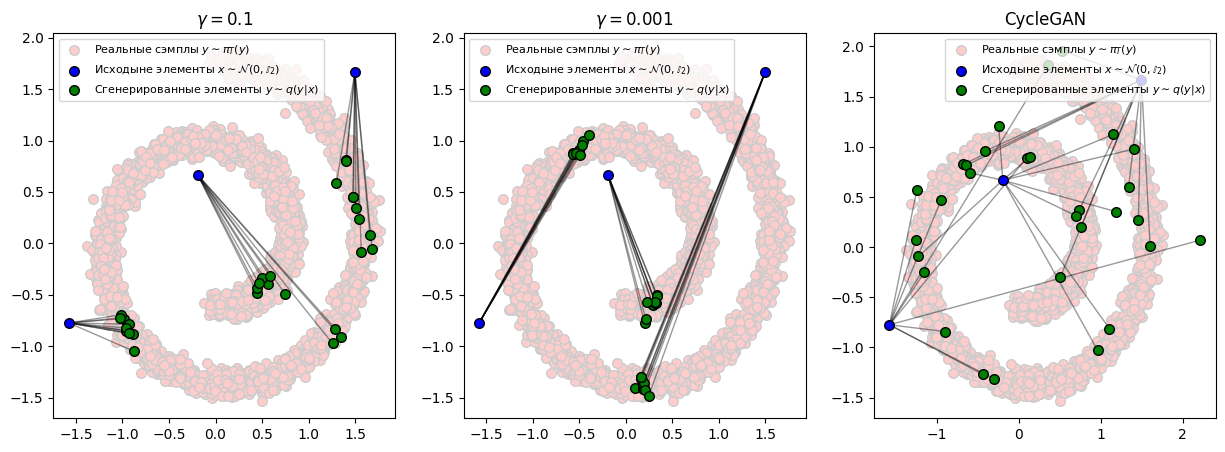
\includegraphics[width=1\linewidth]{slides//4th//figures/2d_gamma.png}
    \end{figure}
\end{frame}

\begin{frame}{EMNIST}
    Эксперимент на EMNIST показывает, что предложенный метод справляется с данными большой размерностью.
    \begin{figure}
        \centering
        \subfloat[Буквы $\rightarrow$ цифры]{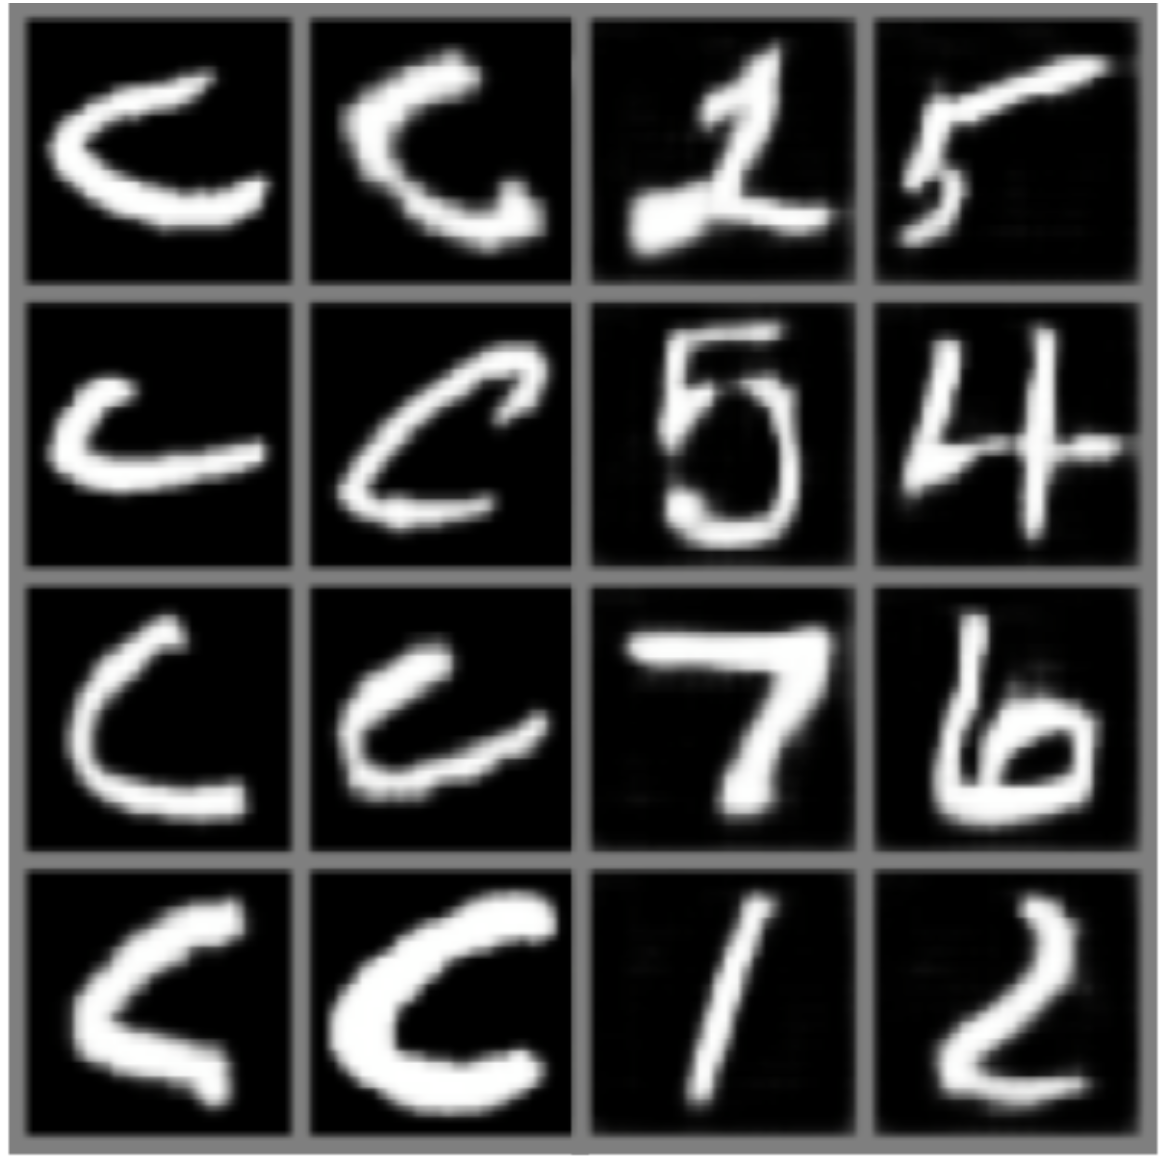
\includegraphics[width=0.4\linewidth]{slides/4th/figures/emnist_cond_p.png}}
        \hfill
        \subfloat[Цифры $\rightarrow$ буквы]{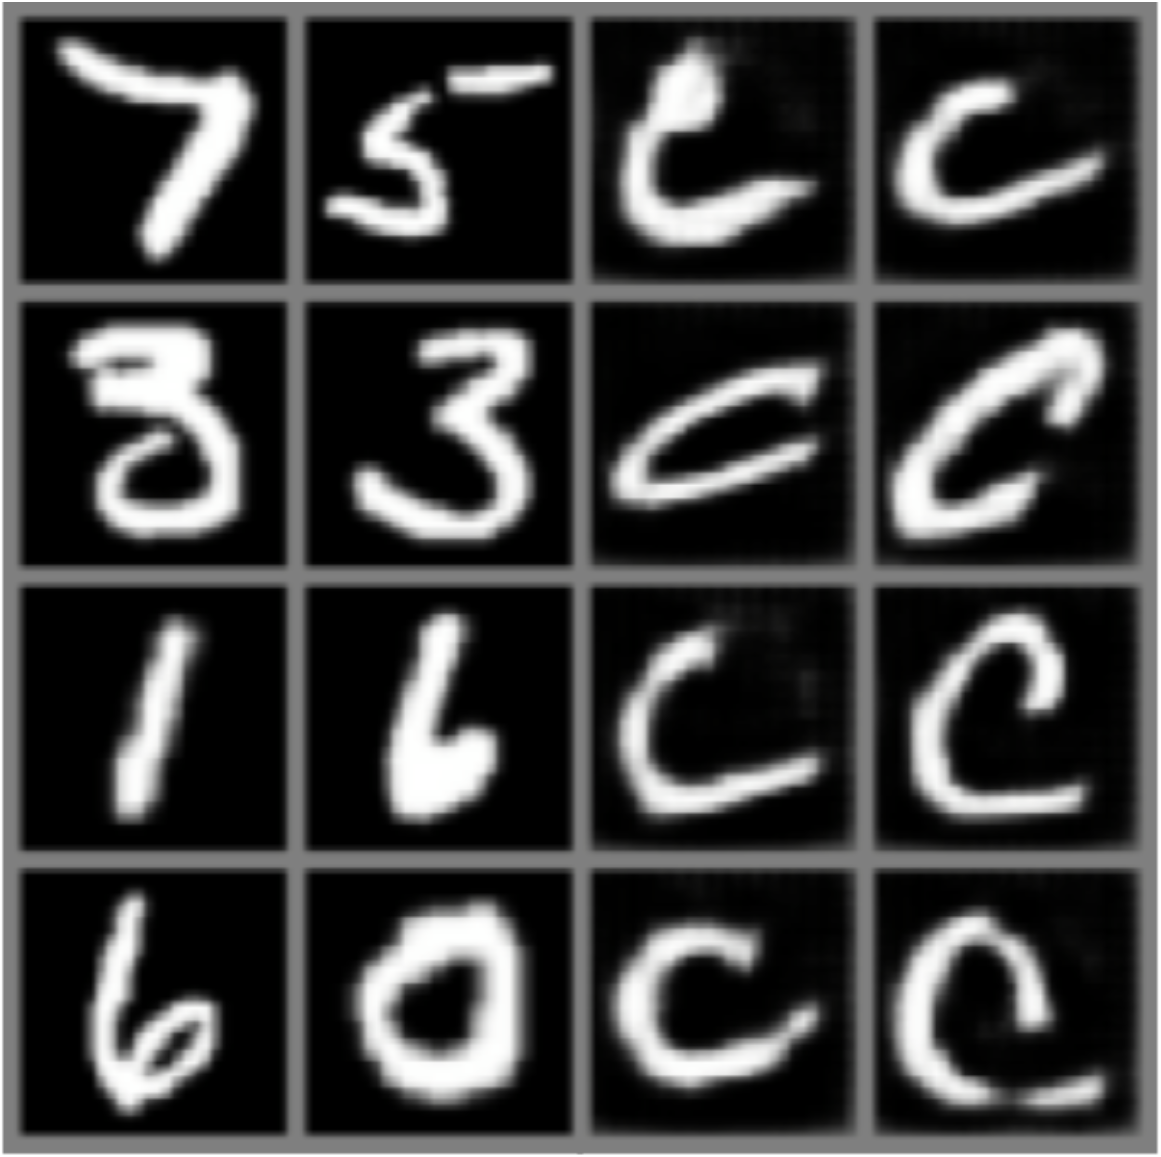
\includegraphics[width=0.4\linewidth]{slides/4th/figures/emnist_cond_q.png}} 
    \end{figure}
\end{frame}
%----------------------------------------------------------------------------------------------------------
\begin{frame}{Выносится на защиту}
    \begin{enumerate}
        \item Предложен новый метод нахождения мостов Шрёдингера, который не моделирует стохастический процесс, а также не обладает проблемой проклятия размерности;
        \item Проведены эксперименты на 2D данных, сравнивающие трансляции с разными $\gamma$;
        \item Проведены эксперименты на 2D данных, сравнивающие предложенный метод с CycleGAN;
        \item Проведены эксперименты на EMNIST, демонстрирующие способность предложенного метода работать с данными большой размерностью.
    \end{enumerate}
\end{frame}
%----------------------------------------------------------------------------------------------------------
\end{document} 